\documentclass{beamer}
\usetheme{Ilmenau}
%\usepackage{longtable}
%\usepackage[flushleft]{threeparttable}
\usepackage{multirow}
\usepackage{array}
\usepackage{comment}
\usepackage{tabu}
\usepackage{longtable}
%\makesavenoteenv{tabular}

%\newcolumntype{K}{>{\centering\arraybackslash}m{3.5cm}}
\setbeamertemplate{navigation symbols}{}
\definecolor{myblue}{rgb}{0.1, 0.2, 0.6}
\setbeamercolor{postit}{fg=white,bg=myblue}
%\setbeamertemplate{footline}[frame number]
%\setbeamertemplate{footline}{%
%   \raisebox{5pt}{\makebox[\paperwidth]{\hfill\makebox[10pt]{\scriptsize\insertframenumber}}}}
%\newcounter{saveenumi}
%\newcommand{\conti}{\setcounter{enumi}{\value{saveenumi}}}
% To increase spaces
%\let\oldframe\frame
%\renewcommand{\frame}{%
%\oldframe
%\let\olditemize\itemize
%\renewcommand\itemize{\olditemize\addtolength{\itemsep}{12pt}}%
%}

%\usepackage{arydshln}
\usepackage{graphicx} % Allows including images
\usepackage{booktabs} % Allows the use of \toprule, \midrule and \bottomrule in tables
\usepackage{caption}
\usepackage{subcaption}
\title[Sex and Education Model \,\,\,\,\,\,\,\,\,\,\,\,\,\,\,\,\,\,\,\,\,\,\,\,\,\,\,\,\,\,\,\,\,\,\,\,\,\,\,\,\,\,\,\,\,\,\,\,\,\,\,\,\,\,\,\,\,\,\,\,\,\,\,\,\,\,\,\,\,\,\,\,\,\,\,\,\,\,\,\,\,\,\,\,\,\,\,\,\,\,\,\,\,\,\,\,\,\,\,\,\,\,\,\,\,\,\,\,\,\,\,\,\,\,\,\,\,\,\,\,\,\,\,\,\,\,\,\,\,\,\,\,\,\,\,\,\,\,\,\,\,\,\,\,\,\,\,\,\,\,\,\,\,\,\,\,\,\,\,\,\,\,\,\,\,\,\,\,\,\,\,\,\,\,\,\,\,\,\,\,\,\,\,\,\,\,\,\,\,\,\,\,\,\,\,\,\,\,\,\,\,\,\,\,\,\,\,\,\,\,\,\,\,\,\,\,\,\,\,\,\,\,\,\,\,\,\,\,\,\,\,\,\insertframenumber/\inserttotalframenumber]{Sex and Education Model: \\Characterizing exposure across the HIV epidemic } % The short title appears at the bottom of every slide, the full title is only on the title page


\author{Christian Aleman}
\institute[UAB-IDEA] % Your institution as it will appear on the bottom of every slide, may be shorthand to save space
{
Advisor: Raul Santaeulalia-Llopis\\
Universitat Aut\`{o}noma de Barcelona \\ 
IDEA-QEM\\% Your institution for the title page
\medskip
\textit{} % Your email address
}
\date{\today} % Date, can be changed to a custom date

\begin{document}


\begin{frame}
\titlepage % Print the title page as the first slide
\end{frame}

\begin{frame}
\tableofcontents
\end{frame}



\section{Introduction}
\subsection{}



\begin{frame}
\frametitle{Introduction: The HIV epidemic in Malawi}
\begin{figure}
  \centering
  \caption{Share of the population infected with HIV}
   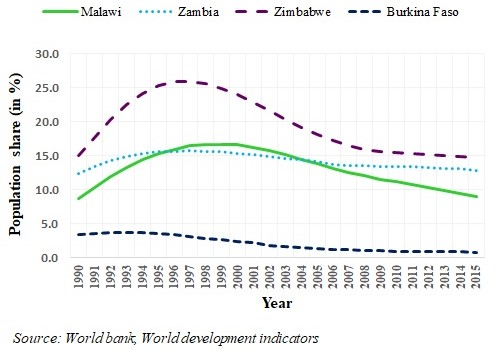
\includegraphics[width=0.75\textwidth]{malawi11.jpg}
 \end{figure}
\end{frame}

\begin{frame}
\frametitle{Introduction: Education and HIV prevalence}
\begin{table}
\centering
\caption{Malawi, HIV prevalence among the general population (in $\%$)}
\label{tablefinal1}
\begin{tabular}{c|c|c|c}
\hline
\multirow{2}{*}{\textbf{}}&\multirow{2}{*}{\textbf{Total}}&\multicolumn{2}{|c}{\textbf{By education level}}\\
\cline{3-4}
 &   &  \textbf{Primary or less}&  \textbf{Secondary or more}\\
 \hline \hline
 DHS 2004& 11.8 & 11.1 & 14.0 \\
 [0.3em]
 DHS 2010    & 10.7 & 10.2 & 11.8 \\
 [0.3em]
\hline \hline
\end{tabular}
\begin{flushleft}
Sources: The prevalences have been taken form DHS data.
\end{flushleft}
\end{table}
\end{frame}





\begin{frame}
\frametitle{Introduction: Relevant literature}
\begin{enumerate}
\item Yao(2016): Promoting education is the most effective way to reduce HIV prevalence.
\item De Walque(2007) fins a negative relation between education and HIV diffusion.
\item Fortson(2008) finds  a positive relation between education risky sex practices.
\item Bledsoe(1990): education only reduces the risk of HIV infection when the health risks are completely understood.

\end{enumerate}
\end{frame}
\begin{frame}
\frametitle{Introduction}

%\setbeamercolor{postit}{fg=black,bg=yellow}
\begin{beamercolorbox}[wd=\textwidth,rounded=true,shadow=true]{postit}
\centering \large Can HIV exposure be characterized by educational differences across epidemic stages?
\end{beamercolorbox}
\vspace{1cm}
\begin{Large}
\begin{itemize}
\item HIV exposure differs across educational groups as the HIV epidemic evolves. Santaeulalia-Llopis $\&$ Iorio (2016)
       
\end{itemize}
\end{Large}

\end{frame}

\begin{frame}
\frametitle{Introduction: The Education Gradient}
\begin{figure}
  \centering
  \caption{The HIV-Education Gradient Across Stages of the Epidemic\footnote{Taken from: Santaeulalia-Llopis $\&$ Iorio (2016)}}
    \begin{subfigure}[b]{0.4\textwidth}
        \centering
        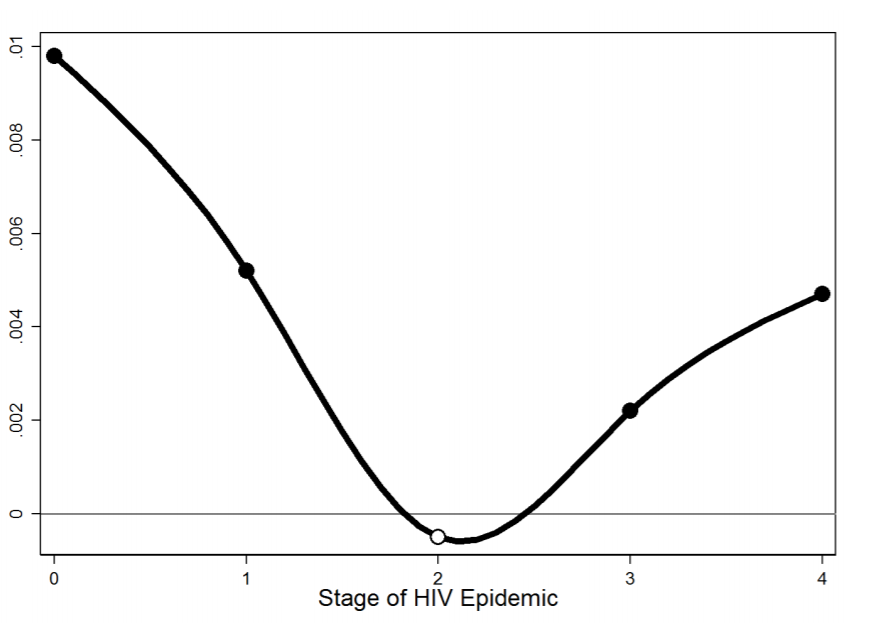
\includegraphics[width=1.3\textwidth]{fig1.png}
        \caption{Whole population}
    \end{subfigure}
    \hfill
      \begin{subfigure}[b]{0.45\textwidth}
        \centering
        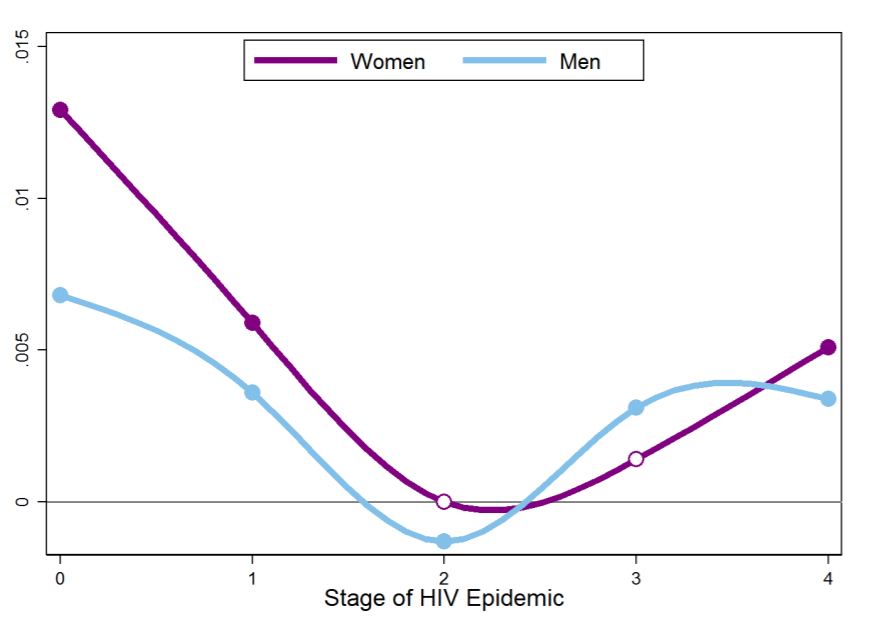
\includegraphics[width=1.2\textwidth]{fig2.png}
        \caption{Gender disaggregation}
    \end{subfigure}
    
\end{figure}
\end{frame}





\section{The Proposed Model}
\subsection{}
\begin{frame}
\frametitle{The Proposed Model:Model characteristics}
%\begin{Large}
\begin{itemize}
\item A Heterogeneous Agent General Equilibrium Model for the Sex market and HIV diffusion.
\item Agents are rational and maximize expected discounted utility subject to a budget constrain.
\item Three markets:
\begin{enumerate}
\item The goods market: \\Agents consume $c$ at price $p_{1}$. 
\item The sex market: \\Non-marital risky sex $x$ is traded for price $p_{2}$.
\item The asset market: \\People save/borrow by trading a non-contingent asset $a$ with return $r$.
\end{enumerate}

\end{itemize}
%\end{Large}
\end{frame}

\begin{frame}
\frametitle{The Proposed Model:More characteristics}
\begin{itemize}
\item Education can be high or low: $E=\{0,1\}$, $e\in E$
\item HIV status can be positive or negative: $H=\{+,-\}$, $h\in H$
\item Individuals can be sex buyers or sex producers $G=\{g,-g\}$
\item $\gamma_{e}$ is the the survival rate. \\ It depends on the level of education $e$ where $\gamma_{1}>\gamma_{0}$.
\item $\psi$ is the fertility rate.
\item Labor is supplied inelastically.
\item Agents earn labor income $y(e)$. \\ y(e) depends on the level of education $e$ where $y(1)>y(0)$.
\end{itemize}

\end{frame}

\begin{frame}
\frametitle{The Proposed Model: Stages of the epidemic}
\Large{\begin{enumerate}
\item Pre-epidemic Stage
\item Myopic Onset of the Epidemic
\item Diffusion and Maturity of the Epidemic
\item ARTs
\end{enumerate}}
\end{frame}

\begin{frame}
\frametitle{1.Pre-Epidemic Stage: No infection}
Here agents differ in gender, assets, educational level.
\begin{itemize}
\item The dynamic problem for sex buyers($g$):

\begin{align*}
V(a,e,g;\Phi) = \max_{c\geq 0,x \geq 0,a' \geq 0} \quad &  u(c,x) + \beta \gamma_e V(a',e,g;\Phi') 
\end{align*}
\begin{align*}
c+ px +a'&= y(e) + (1+r(\Phi))a 
\end{align*}

\item The dynamic problem for sex producers($-g$):

\begin{align*}
V(a,e,-g;\Phi) = \max_{c \geq 0,l \in [0,1],a'\geq 0} \quad &  u(c) + \beta \gamma_e V(a',e,-g;\Phi') 
\end{align*}
\begin{align*}
c +a'&= pl^{\alpha} + y(e)(1-l) + (1+r(\Phi))a  
\end{align*}

\end{itemize}
\end{frame}

\begin{frame}
\frametitle{The aggregate state variable }
The aggregate state evolves according to,
\begin{align*}
\Phi' & = F(\Phi) 
\end{align*}
And define the transition function $Q:\mathcal{Z}\times\mathcal{B(Z)}\to[0,1]$ as: 
\begin{align*}
Q((a,e,g)(\mathcal{A},\mathcal{E},\mathcal{G})) = \left\{
\begin{tabular}{clc}
$\gamma_{e}$ & if      & $a(a,e,g;\Phi) \in \mathcal{A} $\\
0 & else & 
\end{tabular}
\right.
\end{align*}
Then, the evolution of the asset distribution is:
\begin{footnotesize}
\begin{align*}
\Phi'(\mathcal{A},\mathcal{E},\mathcal{G}) = F(\Phi) (\mathcal{A},\mathcal{E},\mathcal{G})= \int_{a,e,g} Q((a,e,g)(\mathcal{A},\mathcal{E},\mathcal{G})) d \Phi+\psi\Phi((a',e,g)(\mathcal{A},\mathcal{E},\mathcal{G}))
\end{align*}
\end{footnotesize}

\end{frame}

\begin{frame}
\frametitle{Solution}
\begin{itemize}
\item Given prices $p,r$ the solution for agents of type $g$ and $-g$  are the policy functions $a(a,e,g;\Phi), x(a,e,g;\Phi), c(a,e,g;\Phi), l(a,e,g;\Phi)$ that induce a stationary distribution $\Phi(\mathcal{A,E,G})$.
\item Market clearing implies:
\begin{align*}
\int_{a,e,g} a(a,e,g;\Phi) d\Phi &= 0 \\
\int_{a,e,g} x (a,e,g;\Phi) d \Phi &= \int_{a,e,g} x(a,e,-g;\Phi) d\Phi
\end{align*}
\end{itemize}



\end{frame}



\begin{frame}
\frametitle{2.Myopic Onset of the Epidemic}

\begin{itemize}
\item People can get infected with HIV at a rate $\lambda(x,h)$ which depends on the amount extramarital risky sex $x$  and the HIV status of the individual $h$. \\Where $\lambda(x,h)$ for $h=0$ takes the form:\footnote{for simplicity define $\lambda(x,0)=\lambda(x)$}\\
\begin{align*}
\lambda(x,0)=\frac{exp(x)}{exp(x)+\rho*exp(-x)}, \,\,\,\,\mbox{where:} \,\,\,\, \frac{\partial\lambda(x)}{\partial x}>0,\frac{\partial\lambda(x)}{\partial \rho}<0
\end{align*}
\item Infected agents earn and might live less: For given $e$, $\gamma_{e}(0)>\gamma_{e}(1)$ and $y(e,0)>y(e,1)$. 
\item Agents are myopic: This is agents are not aware of the risk of getting HIV infected. 
\end{itemize}
\end{frame}


\begin{frame}
\frametitle{2.Myopic Onset of the Epidemic}
\begin{itemize}
\item The dynamic problem for sex buyers($g$):
\begin{footnotesize}
\begin{align*}
V(a,e,g,h;\Phi) = \max_{c,x,a'} \quad &  u(c,x) + \beta \sum_{h'|h} \gamma_e(h') \lambda(x,h'|h) V(a',e,g,h';\Phi)\\
c+ px +a'&= y(e,h) + (1+r(\Phi))a 
\end{align*}
\end{footnotesize}

\item The dynamic problem for sex producers($-g$):
\begin{footnotesize}
\begin{align*}
V(a,e,-g,h;\Phi) = \max_{c,l,a'} \quad &  u(c) + \beta  \sum_{h'|h} \gamma_e(h') \lambda(x,h'|h)  V(a',e,-g,h';\Phi)\\
c +a'&= pl^{\alpha} + y(e,h)(1-l) + (1+r(\Phi))a  
\end{align*}
\item Agents are myopic: they think $h'=0$, so they set the continuation value:
\begin{align*}
V(a',e,g,h'=0;\Phi)\,\,\, \,\,\,\mbox{for}\,\,\, g,-g\in G
\end{align*}
\end{footnotesize}
\end{itemize}
\end{frame}

\begin{frame}
\frametitle{The aggregate state variable }
Define:
\begin{align*}
   \Gamma=
  \left[ {\begin{array}{cc}
   \gamma_{e}(0) & 0 \\
   0 & \gamma_{e}(1) \\
  \end{array} } \right]
   \Lambda=
  \left[ {\begin{array}{cc}
   1-\lambda(x) & 0 \\
   \lambda(x) & 1 \\
  \end{array} } \right]
   \Psi=
  \left[ {\begin{array}{cc}
   \hat{\psi^{0}} & 0 \\
   0 & \hat{\psi^{1}} \\
  \end{array} } \right]
\end{align*}
Then the evolution of the population with education $e$  follows:
\begin{align*}
\left[ {\begin{array}{c}
   \phi_{t+1}(a_{t},e,g,0)\\
   \phi_{t+1}(a_{t},e,g,1)\\
  \end{array} } \right]=\Psi\times \Lambda \times \Gamma\times 
\left[ {\begin{array}{c}
   \phi_{t}(a_{t},e,g,0)\\
   \phi_{t}(a_{t},e,g,1) \\
  \end{array} } \right] 
\end{align*}
Define:
\begin{align*}
\Lambda \times \Gamma=
\left[ {\begin{array}{cc}
   (1-\lambda(x))\gamma_{e}(0)&0\\
   \lambda(x)\gamma_{e}(0)&\gamma_{e}(1)\\
  \end{array} } \right]=\Omega
\end{align*}





\end{frame}

\begin{frame}
Then, together with the decision rule $a(a,e,g,h,\Phi)$ the transition matrix $\mathcal{Q}((a,e,g,h)(\mathcal{A,E,G,H}))$is constructed as follows:
\begin{align*}
\mathcal{Q}((a,e,g,h)(\mathcal{A,E,G,H}))=\sum_{h'\in \mathcal{H}}\textbf{1}_{a\in \mathcal{A}} \Omega(h'|h)
\end{align*} 
And the endogenous asset distribution can be rewritten as: 
\begin{footnotesize}
\begin{align*}
\boldsymbol{\phi}_{t+1}(a_{t+1},e,g,h_{t+1})=\int_{a,e,g,h}\sum_{h_{t+1}|h_{t}}&\textbf{1}_{a_{t+1}=a(a,e,g,h)}\gamma_{e}(h_{t+1})\lambda_{e}(h_{t+1}|h_{t})d \boldsymbol{\phi}_{t}(a,e,g,h) \nonumber\\
&+\psi\boldsymbol{\phi}_{t}(a_{t+1},e,g,h_{t+1})
\end{align*} 
\end{footnotesize}

\end{frame}

\begin{frame}
\frametitle{3.Diffusion and Maturity of the Epidemic}
\begin{itemize}
\item Individuals are now aware of the possibility of infection. Educated people ($e=1$) understand the risk more accurately.\\
Then $\rho_{1}>\rho_{0}$.
\item The previous implies that $\lambda_{e}(x,h)$ also depends on the level of education ($e$).
\item The dynamic problems are the same only that now the individuals set the correct continuation value. 
\end{itemize}

\end{frame}

\begin{frame}
\frametitle{4.ARTs}
Drugs are supplied to all infected individuals, Then $h=1 \Rightarrow d=1$\\
Drugs ($d$):
\begin{itemize}
\item Increase survival Rates for the infected $\gamma_{e}(1,d)\Rightarrow\gamma_{e}(1,1)$
\item Increases productivity of the infected $y(e,1,d)\Rightarrow y(e,1,1)$

\end{itemize}
\end{frame}

\begin{frame}
\frametitle{Solution algorithm}
%\begin{enumerate}
%\item 
%\end{enumerate}
\begin{tabular}{p{2cm}p{8cm}}
\textbf{Step 1:}& Find stationary equilibrium for the \underline{\textit{pre-epidemic stage}}.\\
\textbf{Step 2:}& The \underline{\textit{myopic stage}} arrives as an unexpected shock. However agents are not aware of it.\\
& Solve forward using the decision rules of the \underline{\textit{pre-epidemic stage}} but with the productivity level, infection probabilities and survival rates of \underline{\textit{myopic stage}}. \\
\end{tabular}
\end{frame}



\begin{frame}
\frametitle{Solution algorithm continuation}
%\begin{enumerate}
%\item 
%\end{enumerate}
\begin{tabular}{p{2cm}p{8cm}}
\textbf{Step 3:}& \underline{\textit{Maturity}} arrives as an unexpected shock before the \underline{\textit{myopic stage}} reaches a steady state. Find the steady state of the \underline{\textit{maturity stage}}, start solving backwards for the proportion $\mu$ of agents that understand the risks of infection. Solve forward for agents $1-\mu$ who are still myopic. At some point all agents will be aware of the risk. \\
\textbf{Step 4:}& The \underline{\textit{ARTs stage}} arrives as an unexpected shock. Again the \underline{\textit{maturity stage}} never reaches the steady state. First compute the steady state of \underline{\textit{ARTs stage}} and solve backwards until the turning point with the \underline{\textit{maturity stage}} is reached.\\
\end{tabular}
\end{frame}



\section{Calibration}
\subsection{}

\begin{frame}
\frametitle{Calibration}
The model was calibrated to match data from the Malawian HIV epidemic: 
\begin{footnotesize}
\begin{table}
\centering
\caption{Targeted Prevalences (in $\%$) }
\label{tablefinal1}
\begin{tabular}{c|>{\centering\arraybackslash}m{0.7cm}|>{\centering\arraybackslash}m{2cm}|c|c}
\hline
\multirow{2}{*}{\textbf{Stage}}& \multirow{2}{*}{\textbf{Year}} &  \multirow{2}{*}{\textbf{Total}}&  \multicolumn{2}{|>{\centering\arraybackslash}m{4cm}}{\textbf{HIV/AIDS Prevalence of (*) who completed higher education or more}}\\
\cline{4-5}
&&&(*)\textbf{Females}&(*)\textbf{Males}\\
 \hline \hline
 Myopic Stage& 2000 & 15.0 & 19.3 &16.5\\
 [0.3em]
 Maturity    & 2004 & 11.8 & 15.1 &12.9\\
 [0.3em]
 ARTs        & 2010 & 10.7 & 16.1&8.9\\
\hline \hline
\end{tabular}
\begin{flushleft}
Sources: Taken form DHS data.
\end{flushleft}

\end{table}
\end{footnotesize}
\end{frame}

\begin{frame}
\begin{footnotesize}
\begin{table}[H]
\centering
\caption{Fertility and mortality rates}
\label{tablefinal2}
\begin{tabular}{c|c|>{\centering\arraybackslash}m{1.5cm}|>{\centering\arraybackslash}m{2.7cm}|>{\centering\arraybackslash}m{2.7cm}}
\hline
 \textbf{Stage}& \textbf{Year} & \textbf{Fertility rate($\%$)} & \textbf{Mortality rate including HIV/AIDS deaths($\%$)}&\textbf{Mortality rate excluding HIV/AIDS deaths($\%$)} \\
 \hline \hline
 Myopic Stage& 2000 & 6.20 &1.68&1.35\\
 [0.3em]
 Maturity    & 2004 & 5.95 &1.45&1.04\\
 [0.3em]
 ARTs        & 2010 & 5.30 &0.98&0.71\\
 \hline \hline
\end{tabular}
\begin{flushleft}
Sources:  World Bank, Sustainable Development Indicators.
\end{flushleft}
\end{table}
\end{footnotesize}
\end{frame}

\begin{frame}
\begin{footnotesize}
\begin{table}[H]
\centering
\caption{Share of people educated but infected}
\label{tablefinal3}
\begin{tabular}{c|c|c|c|c|c}
\hline
 \multirow{ 2}{*}{\textbf{Stage}}&\multirow{ 2}{*}{\textbf{Year}}&\multicolumn{2}{>{\centering\arraybackslash}m{3.5cm}}{\textbf{Share of (*) with secondary education or more($\%$)}}&\multicolumn{2}{|>{\centering\arraybackslash}m{3.5cm}}{\textbf{Share of (**)with secondary education or more and are infected ($\%$).}\vspace{0.1cm}}\\
 [0.6em]
 \cline{3-6}
  &  & \textbf{(*)Females}&\textbf{(*)Males} &\textbf{(**)Females}&\textbf{(**)Males} \\
 \hline \hline
 Myopic Stage& 2000 &11.1&20.9&2.1&3.4\\
 [0.3em]
 Maturity    & 2004  &15.5&27.2&2.3&3.5\\
 [0.3em]
 ARTs        & 2010 &20.0&31.2 &3.2&2.8\\
 \hline \hline
\end{tabular}
\begin{flushleft}
Sources:  DHS data .
\end{flushleft}
\end{table}
\end{footnotesize}
\end{frame}

\begin{frame}
\frametitle{An additional assumption necessary for the calibration}
\begin{Large}
Assumption about the gender of the individuals:
\begin{itemize}
\item Men are risky sex buyers.
\item Females are risky sex producers.
\item There is no reasons why it couldn't be the other way around.
\end{itemize}
\end{Large}

\end{frame}



\begin{comment}


\begin{frame}
\frametitle{Results}

\begin{figure}
  \centering
  \caption{}
    \begin{subfigure}[b]{0.4\textwidth}
        \centering
        \includegraphics[width=1.3\textwidth]{Pre-Epidemic/fig3.jpg}
      
    \end{subfigure}
    \hfill
      \begin{subfigure}[b]{0.45\textwidth}
        \centering
        \includegraphics[width=1.2\textwidth]{Pre-Epidemic/fig4.jpg}
       
    \end{subfigure}
    
\end{figure}

\end{frame}

\begin{frame}
\frametitle{Results}

\begin{figure}
  \centering
  \caption{}
    \begin{subfigure}[b]{0.4\textwidth}
        \centering
        \includegraphics[width=1.3\textwidth]{Pre-Epidemic/fig5.jpg}
      
    \end{subfigure}
    \hfill
      \begin{subfigure}[b]{0.45\textwidth}
        \centering
        \includegraphics[width=1.2\textwidth]{Pre-Epidemic/fig6.jpg}
       
    \end{subfigure}
    
\end{figure}

\end{frame}
\begin{frame}
\frametitle{Results}

\begin{figure}
  \centering
  \caption{}
    \begin{subfigure}[b]{0.4\textwidth}
        \centering
        \includegraphics[width=1.3\textwidth]{Pre-Epidemic/fig7.jpg}
      
    \end{subfigure}
    \hfill
      \begin{subfigure}[b]{0.45\textwidth}
        \centering
        \includegraphics[width=1.2\textwidth]{Pre-Epidemic/fig8.jpg}
       
    \end{subfigure}
    
\end{figure}

\end{frame}

\begin{frame}
\frametitle{Results}

\begin{figure}
  \centering
  \caption{}
    \begin{subfigure}[b]{0.4\textwidth}
        \centering
        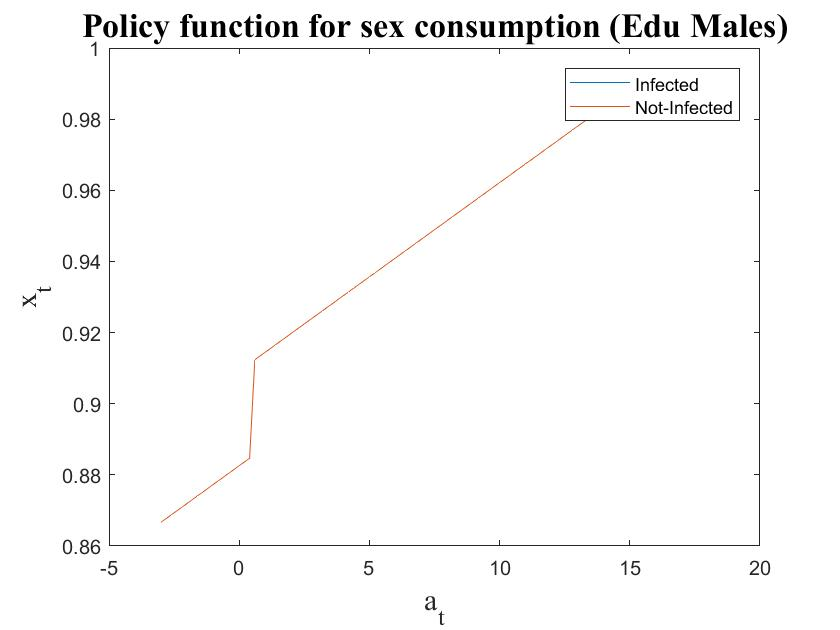
\includegraphics[width=1.3\textwidth]{Pre-Epidemic/fig9.jpg}
      
    \end{subfigure}
    \hfill
      \begin{subfigure}[b]{0.45\textwidth}
        \centering
        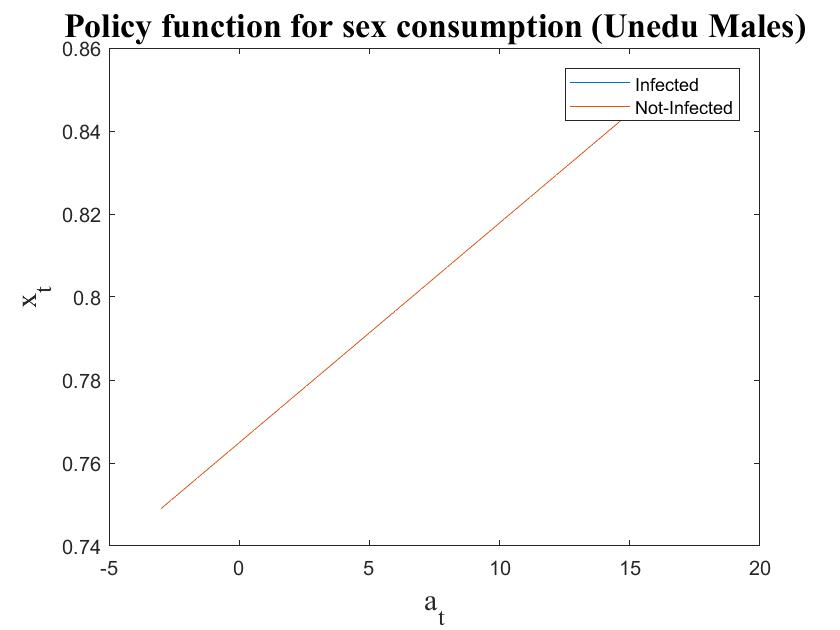
\includegraphics[width=1.2\textwidth]{Pre-Epidemic/fig10.jpg}
       
    \end{subfigure}
    
\end{figure}

\end{frame}

\begin{frame}
\frametitle{Results}

\begin{figure}
  \centering
  \caption{}
    \begin{subfigure}[b]{0.4\textwidth}
        \centering
        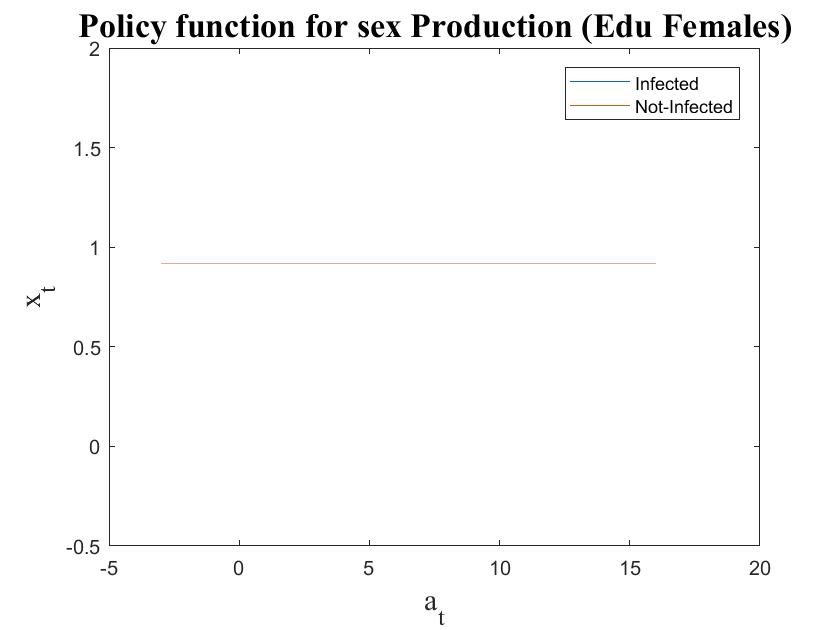
\includegraphics[width=1.3\textwidth]{Pre-Epidemic/fig11.jpg}
      
    \end{subfigure}
    \hfill
      \begin{subfigure}[b]{0.45\textwidth}
        \centering
        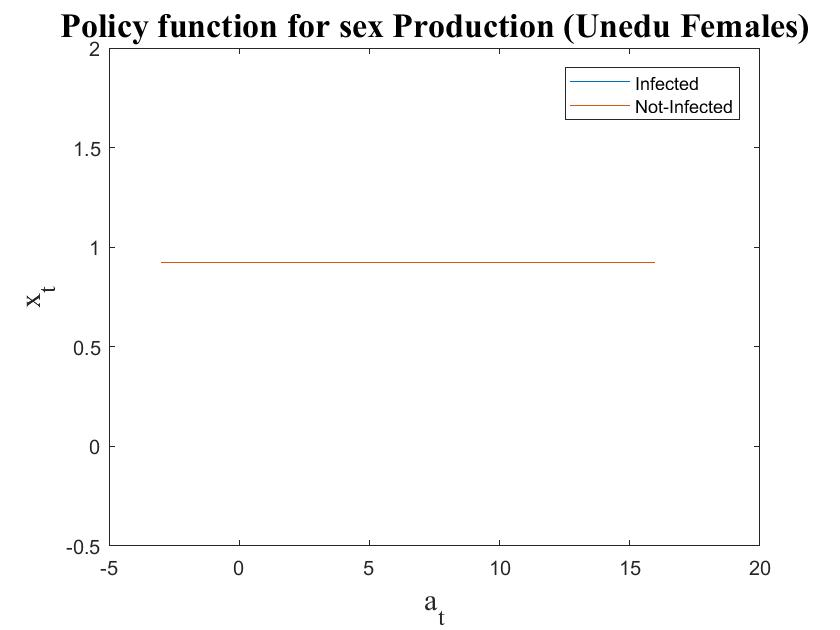
\includegraphics[width=1.2\textwidth]{Pre-Epidemic/fig12.jpg}
       
    \end{subfigure}
    
\end{figure}

\end{frame}



\section{Miopic}

\begin{frame}
\frametitle{Results}

\begin{figure}
  \centering
  \caption{}
    \begin{subfigure}[b]{0.4\textwidth}
        \centering
        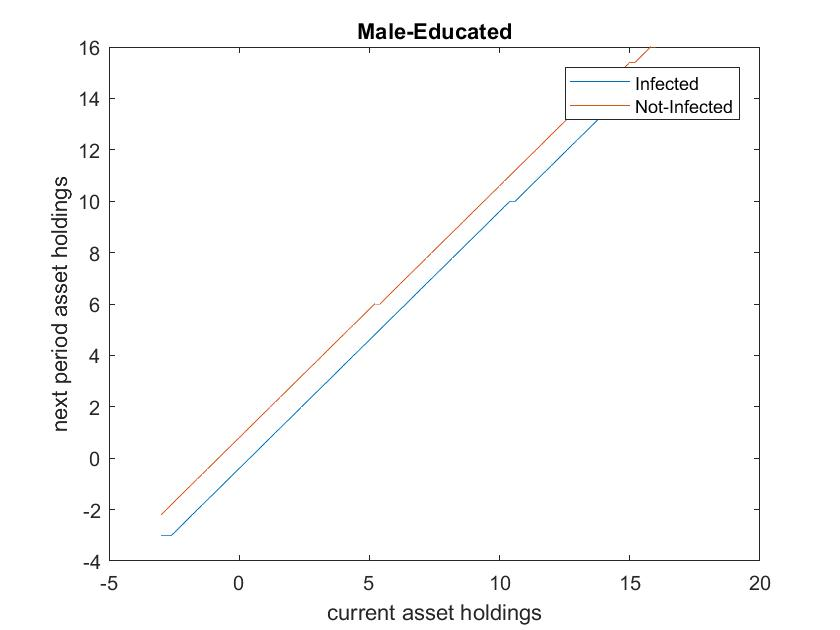
\includegraphics[width=1.3\textwidth]{miopic/fig1m.jpg}
      
    \end{subfigure}
    \hfill
      \begin{subfigure}[b]{0.45\textwidth}
        \centering
        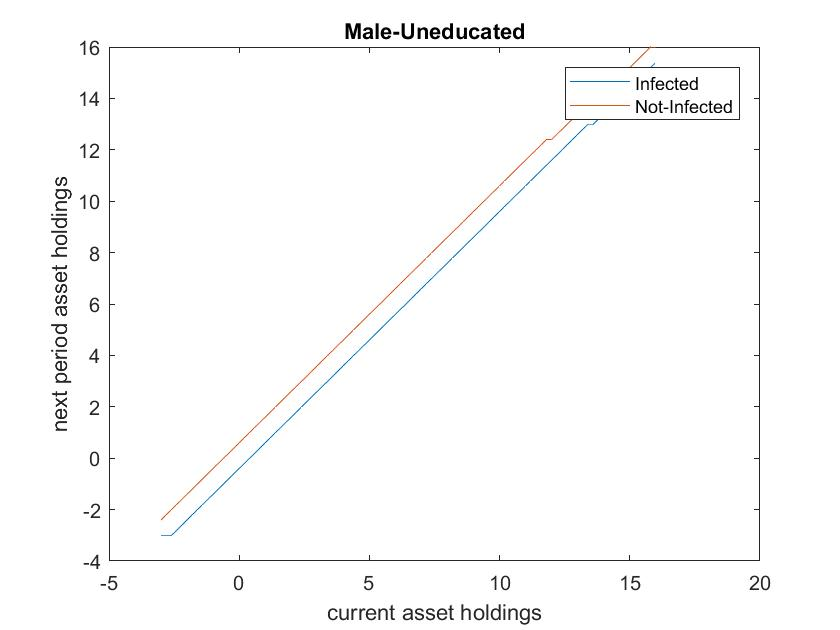
\includegraphics[width=1.2\textwidth]{miopic/fig2m.jpg}
       
    \end{subfigure}
    
\end{figure}

\end{frame}

\begin{frame}
\frametitle{Results}
%\begin{itemize}

\begin{figure}
  \centering
  \caption{}
    \begin{subfigure}[b]{0.4\textwidth}
        \centering
        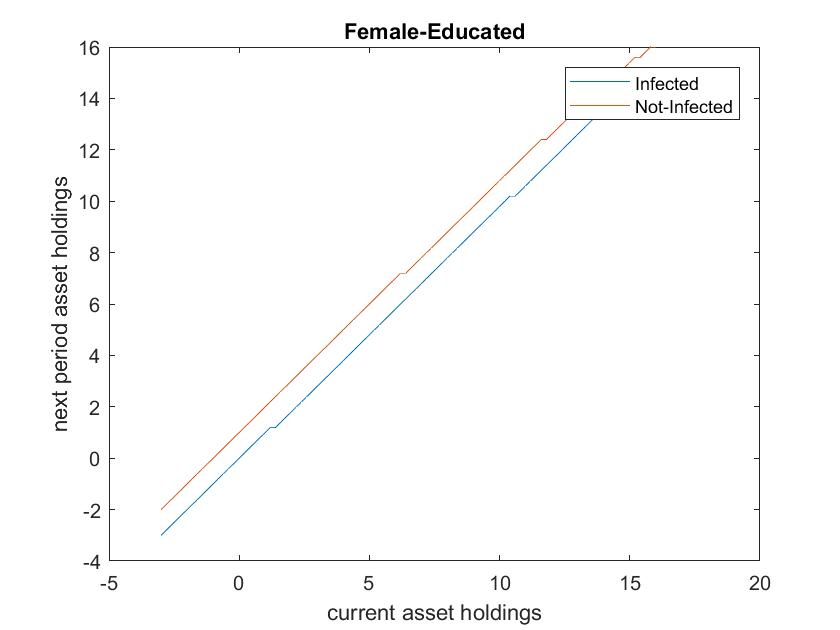
\includegraphics[width=1.3\textwidth]{miopic/fig3m.jpg}
      
    \end{subfigure}
    \hfill
      \begin{subfigure}[b]{0.45\textwidth}
        \centering
        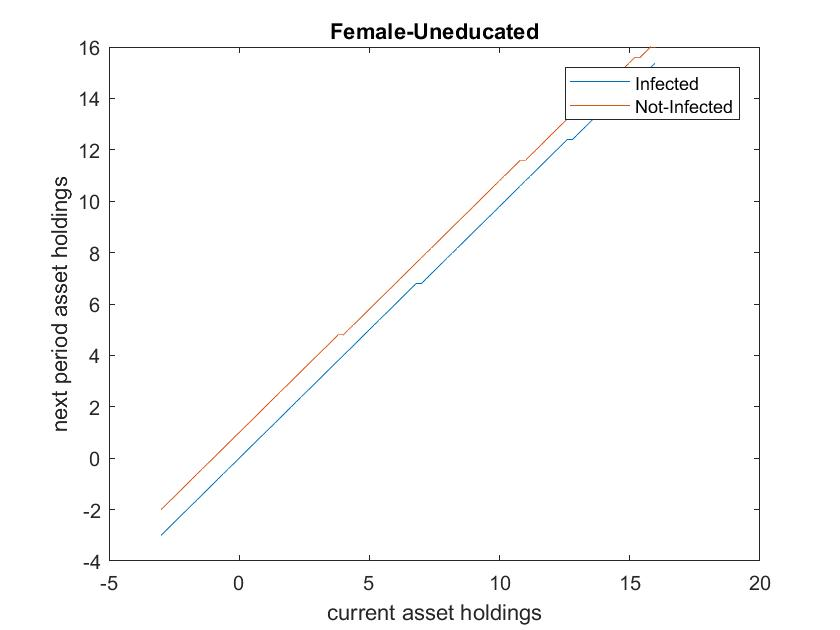
\includegraphics[width=1.2\textwidth]{miopic/fig4m.jpg}
       
    \end{subfigure}
    
\end{figure}

%\end{itemize}
\end{frame}
\begin{frame}
\frametitle{Results}

\begin{figure}
  \centering
  \caption{}
    \begin{subfigure}[b]{0.4\textwidth}
        \centering
        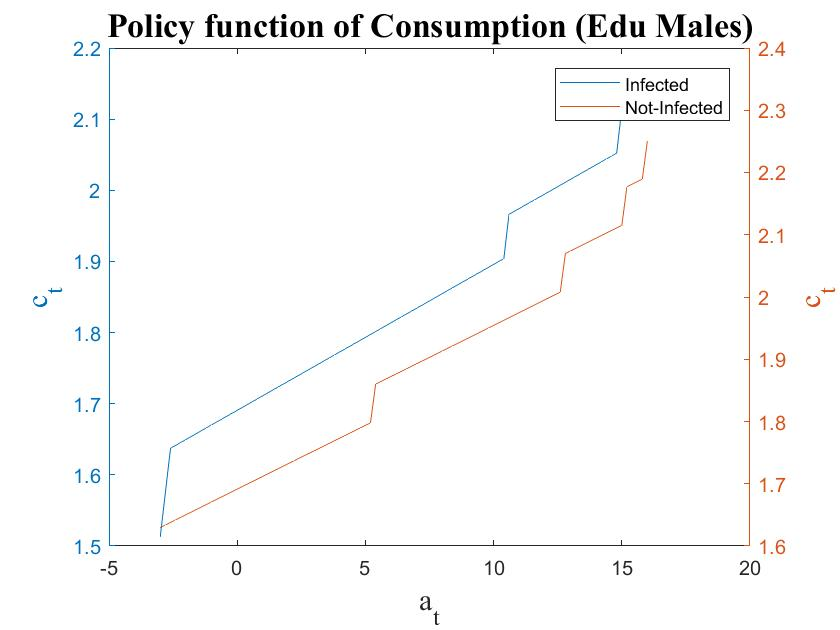
\includegraphics[width=1.3\textwidth]{miopic/fig5m.jpg}
      
    \end{subfigure}
    \hfill
      \begin{subfigure}[b]{0.45\textwidth}
        \centering
        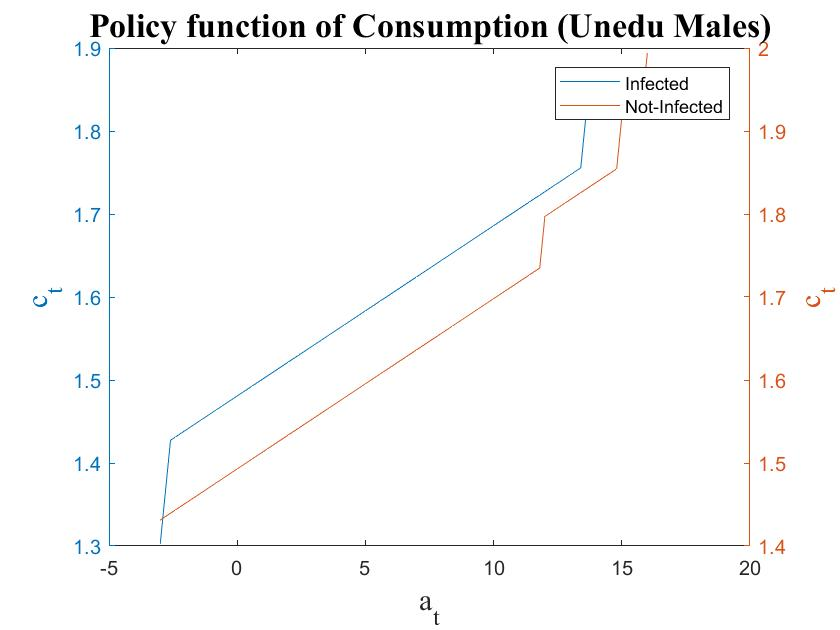
\includegraphics[width=1.2\textwidth]{miopic/fig6m.jpg}
       
    \end{subfigure}
    
\end{figure}
\end{frame}

\begin{frame}
\frametitle{Results}

\begin{figure}
  \centering
  \caption{}
    \begin{subfigure}[b]{0.4\textwidth}
        \centering
        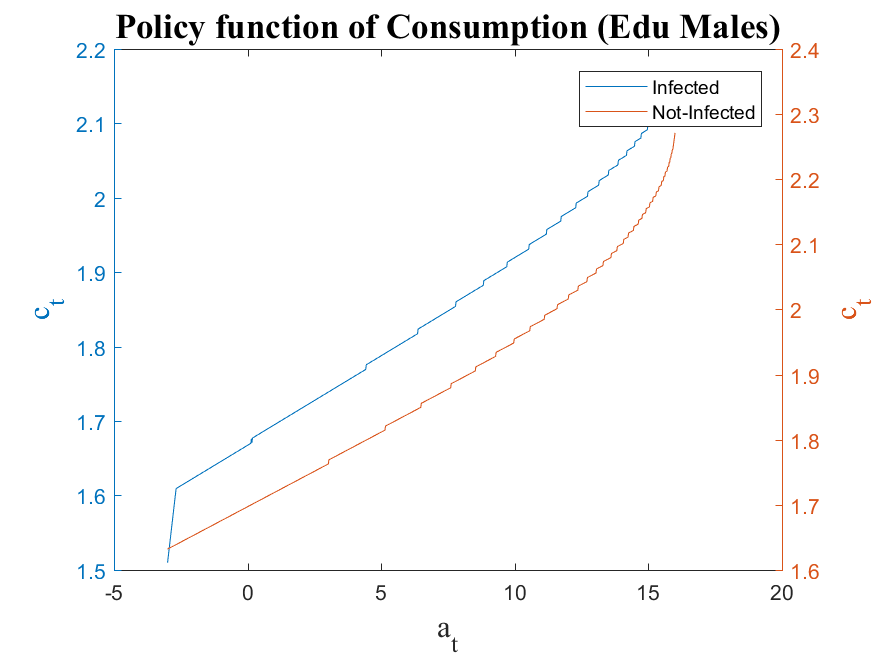
\includegraphics[width=1.3\textwidth]{miopics1/FIG5.png}
      
    \end{subfigure}
    \hfill
      \begin{subfigure}[b]{0.45\textwidth}
        \centering
        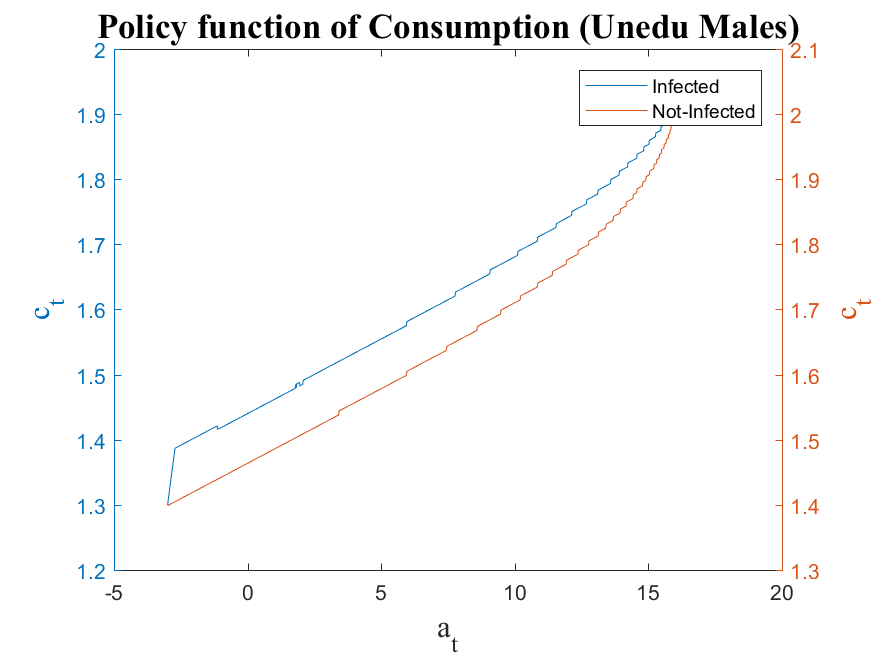
\includegraphics[width=1.2\textwidth]{miopics1/FIG6.png}
       
    \end{subfigure}
    
\end{figure}
\end{frame}


\begin{frame}
\frametitle{Results}

\begin{figure}
  \centering
  \caption{}
    \begin{subfigure}[b]{0.4\textwidth}
        \centering
        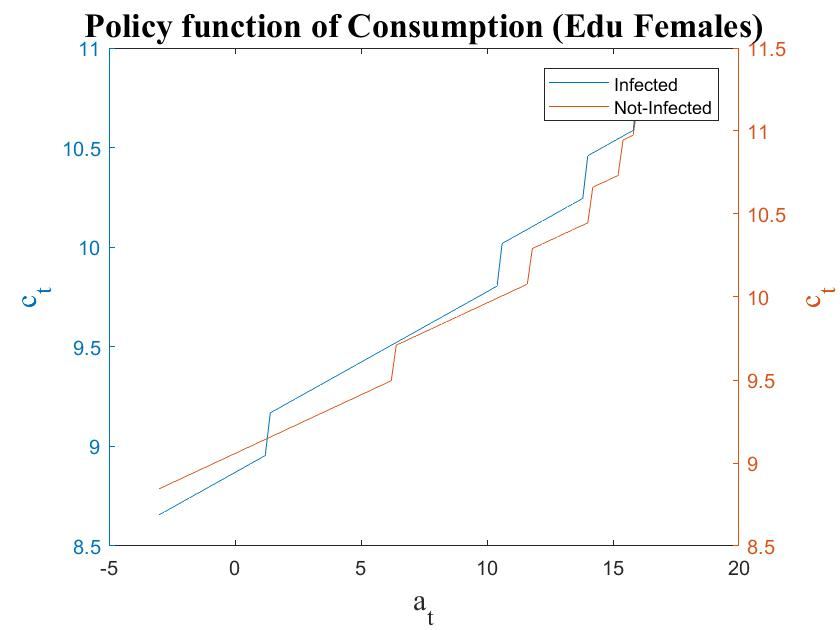
\includegraphics[width=1.3\textwidth]{miopic/fig7m.jpg}
      
    \end{subfigure}
    \hfill
      \begin{subfigure}[b]{0.45\textwidth}
        \centering
        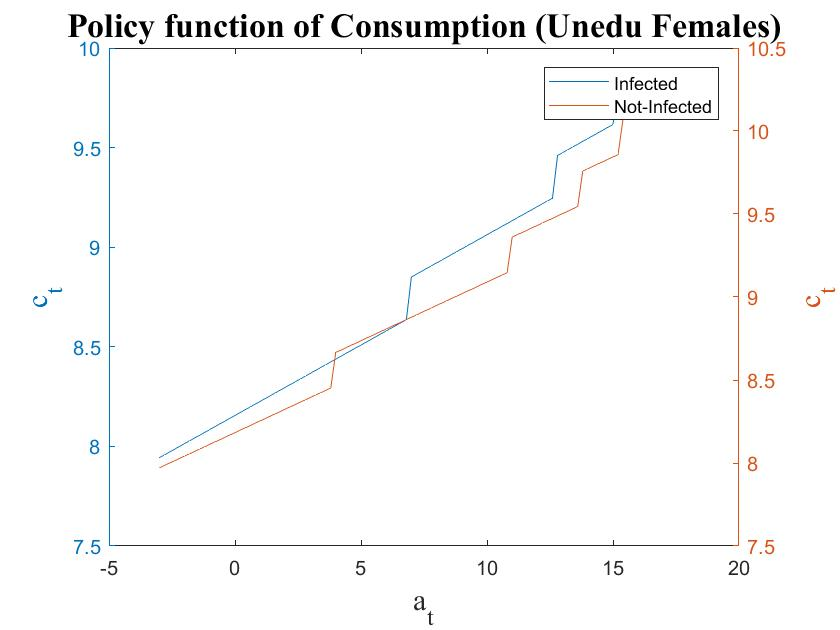
\includegraphics[width=1.2\textwidth]{miopic/fig8m.jpg}
       
    \end{subfigure}
    
\end{figure}

\end{frame}

\begin{frame}
\frametitle{Results}
%\begin{itemize}

\begin{figure}
  \centering
  \caption{}
    \begin{subfigure}[b]{0.4\textwidth}
        \centering
        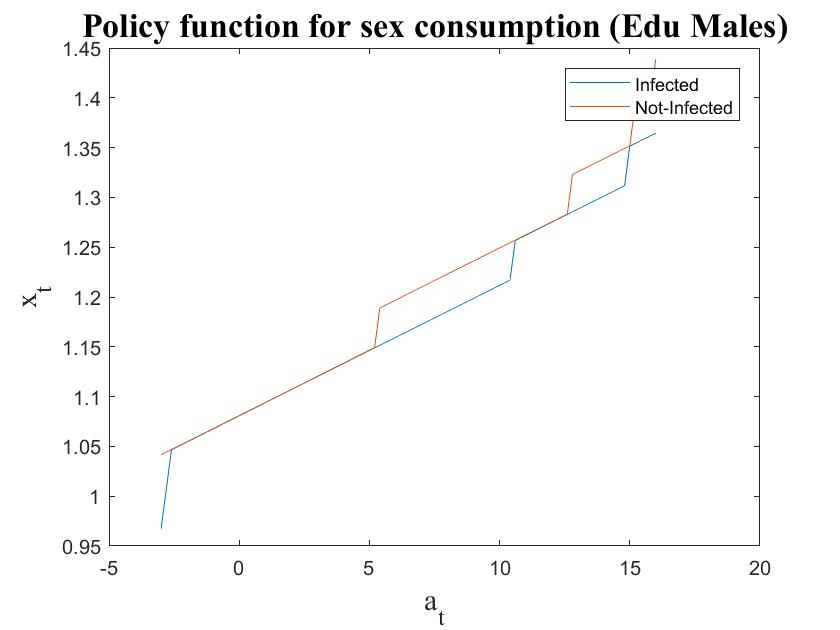
\includegraphics[width=1.3\textwidth]{miopic/fig9m.jpg}
      
    \end{subfigure}
    \hfill
      \begin{subfigure}[b]{0.45\textwidth}
        \centering
        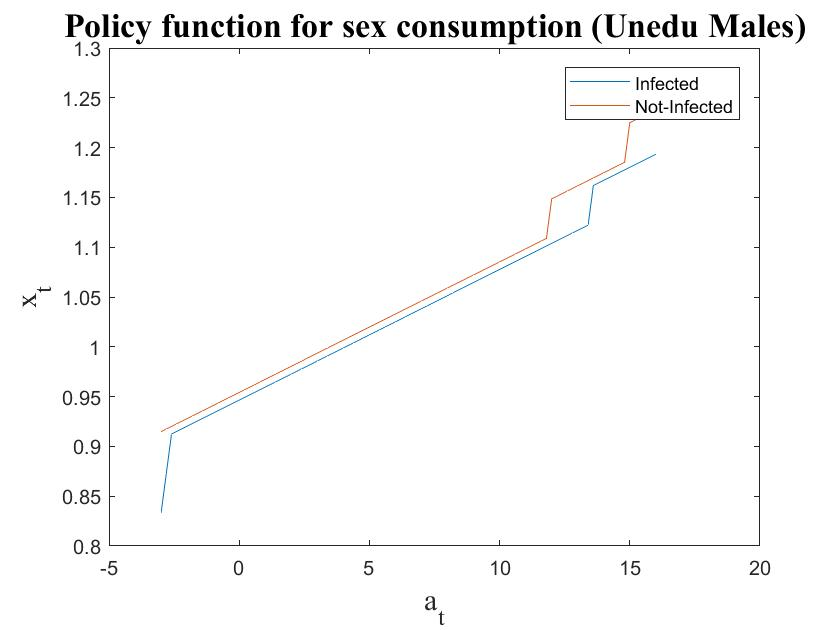
\includegraphics[width=1.2\textwidth]{miopic/fig10m.jpg}
       
    \end{subfigure}
    
\end{figure}

%\end{itemize}
\end{frame}
\begin{frame}
\frametitle{Results}

\begin{figure}
  \centering
  \caption{}
    \begin{subfigure}[b]{0.4\textwidth}
        \centering
        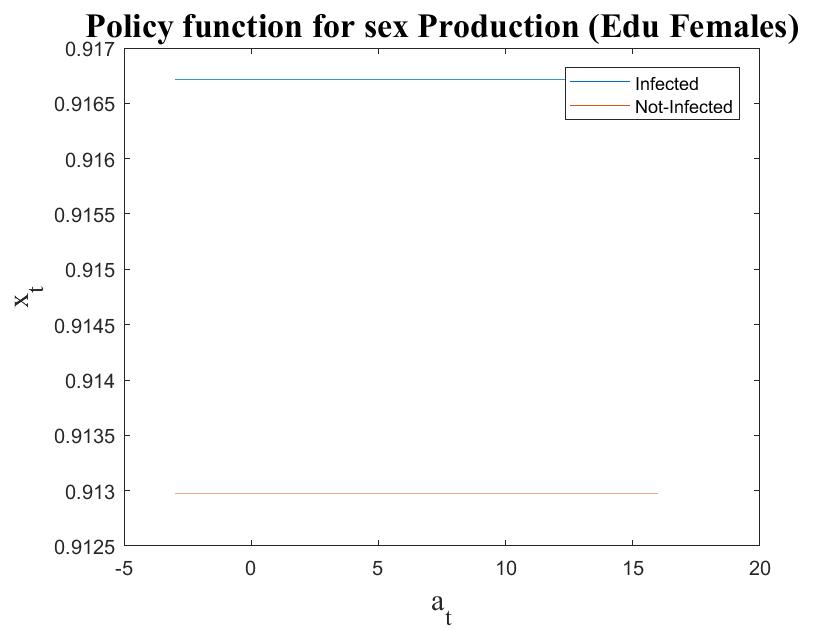
\includegraphics[width=1.3\textwidth]{miopic/fig11m.jpg}
      
    \end{subfigure}
    \hfill
      \begin{subfigure}[b]{0.45\textwidth}
        \centering
        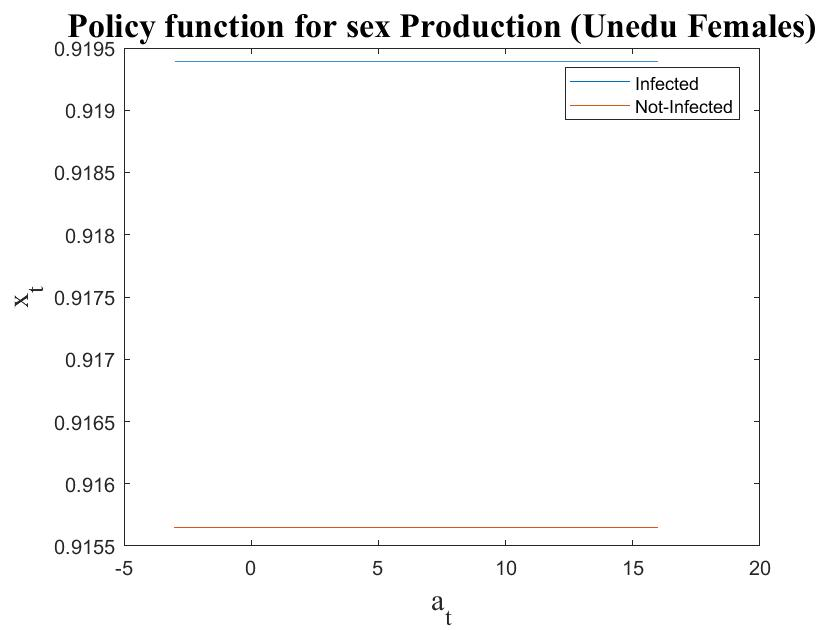
\includegraphics[width=1.2\textwidth]{miopic/fig12m.jpg}
       
    \end{subfigure}
    
\end{figure}


\end{frame}



\section{Onset of the epidemic}


\begin{frame}
\frametitle{Results}

\begin{figure}
  \centering
  \caption{}
    \begin{subfigure}[b]{0.4\textwidth}
        \centering
        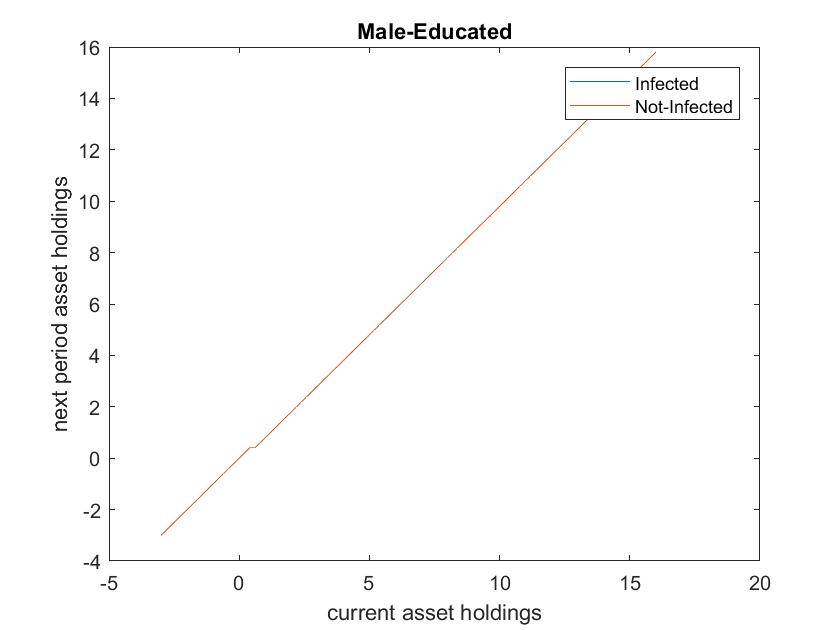
\includegraphics[width=1.3\textwidth]{miopics/fig1.jpg}
      
    \end{subfigure}
    \hfill
      \begin{subfigure}[b]{0.45\textwidth}
        \centering
        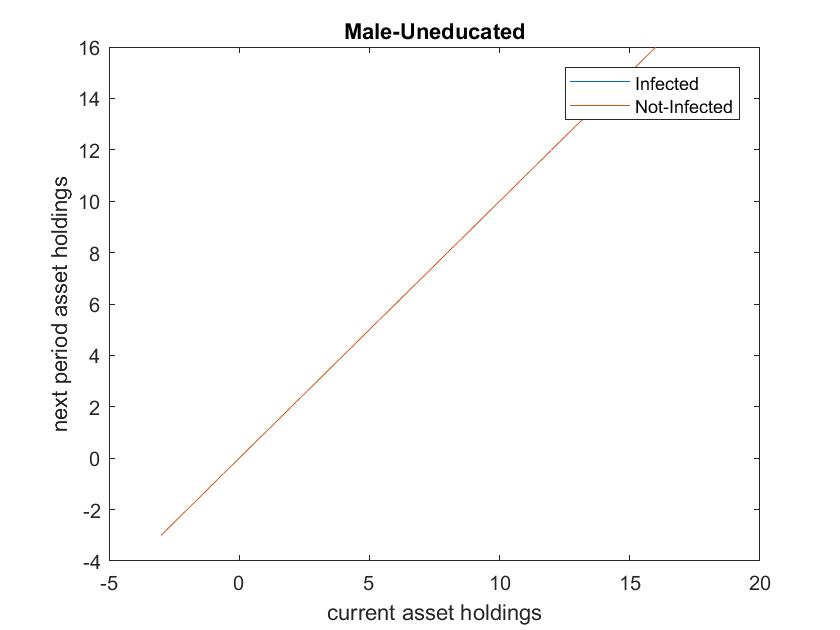
\includegraphics[width=1.2\textwidth]{miopics/fig2.jpg}
       
    \end{subfigure}
    
\end{figure}


\end{frame}


\begin{frame}
\frametitle{Results}

\begin{figure}
  \centering
  \caption{}
    \begin{subfigure}[b]{0.4\textwidth}
        \centering
        \includegraphics[width=1.3\textwidth]{miopics/fig3.jpg}
      
    \end{subfigure}
    \hfill
      \begin{subfigure}[b]{0.45\textwidth}
        \centering
        \includegraphics[width=1.2\textwidth]{miopics/fig4.jpg}
       
    \end{subfigure}
    
\end{figure}


\end{frame}


\begin{frame}
\frametitle{Results}

\begin{figure}
  \centering
  \caption{}
    \begin{subfigure}[b]{0.4\textwidth}
        \centering
        \includegraphics[width=1.3\textwidth]{miopics/fig5.jpg}
      
    \end{subfigure}
    \hfill
      \begin{subfigure}[b]{0.45\textwidth}
        \centering
        \includegraphics[width=1.2\textwidth]{miopics/fig6.jpg}
       
    \end{subfigure}
    
\end{figure}


\end{frame}

\begin{frame}
\frametitle{Results}

\begin{figure}
  \centering
  \caption{}
    \begin{subfigure}[b]{0.4\textwidth}
        \centering
        \includegraphics[width=1.3\textwidth]{miopics/fig7.jpg}
      
    \end{subfigure}
    \hfill
      \begin{subfigure}[b]{0.45\textwidth}
        \centering
        \includegraphics[width=1.2\textwidth]{miopics/fig8.jpg}
       
    \end{subfigure}
    
\end{figure}


\end{frame}


\begin{frame}
\frametitle{Results}

\begin{figure}
  \centering
  \caption{}
    \begin{subfigure}[b]{0.4\textwidth}
        \centering
        \includegraphics[width=1.3\textwidth]{miopics/figo8.jpg}
      
    \end{subfigure}
    \hfill
      \begin{subfigure}[b]{0.45\textwidth}
        \centering
        \includegraphics[width=1.2\textwidth]{miopics/figo10.jpg}
       
    \end{subfigure}
    
\end{figure}


\end{frame}


\begin{frame}
\frametitle{Results}

\begin{figure}
  \centering
  \caption{}
    \begin{subfigure}[b]{0.4\textwidth}
        \centering
        \includegraphics[width=1.3\textwidth]{miopics/figo11.jpg}
      
    \end{subfigure}
    \hfill
      \begin{subfigure}[b]{0.45\textwidth}
        \centering
        \includegraphics[width=1.2\textwidth]{miopics/figo12.jpg}
       
    \end{subfigure}
    
\end{figure}


\end{frame}

\section{ART}
\begin{frame}
\frametitle{Results}

\begin{figure}
  \centering
  \caption{}
    \begin{subfigure}[b]{0.4\textwidth}
        \centering
        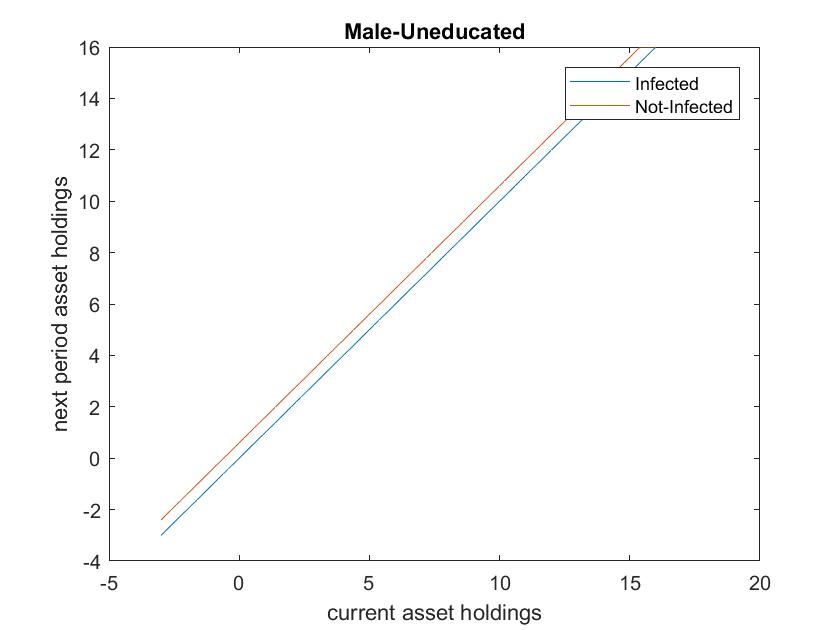
\includegraphics[width=1.3\textwidth]{miopicss/fig1a.jpg}
      
    \end{subfigure}
    \hfill
      \begin{subfigure}[b]{0.45\textwidth}
        \centering
        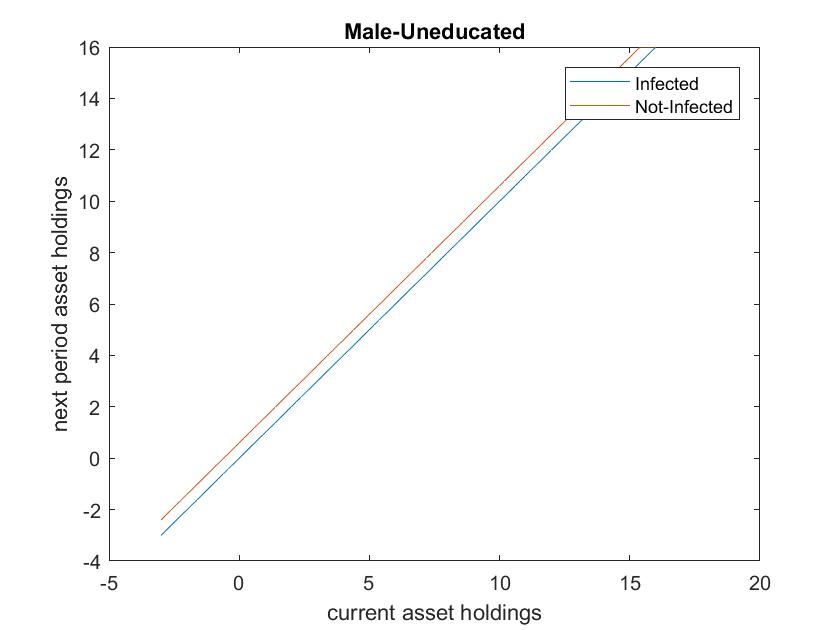
\includegraphics[width=1.2\textwidth]{miopicss/fig2a.jpg}
       
    \end{subfigure}
    
\end{figure}


\end{frame}

\begin{frame}
\frametitle{Results}

\begin{figure}
  \centering
  \caption{}
    \begin{subfigure}[b]{0.4\textwidth}
        \centering
        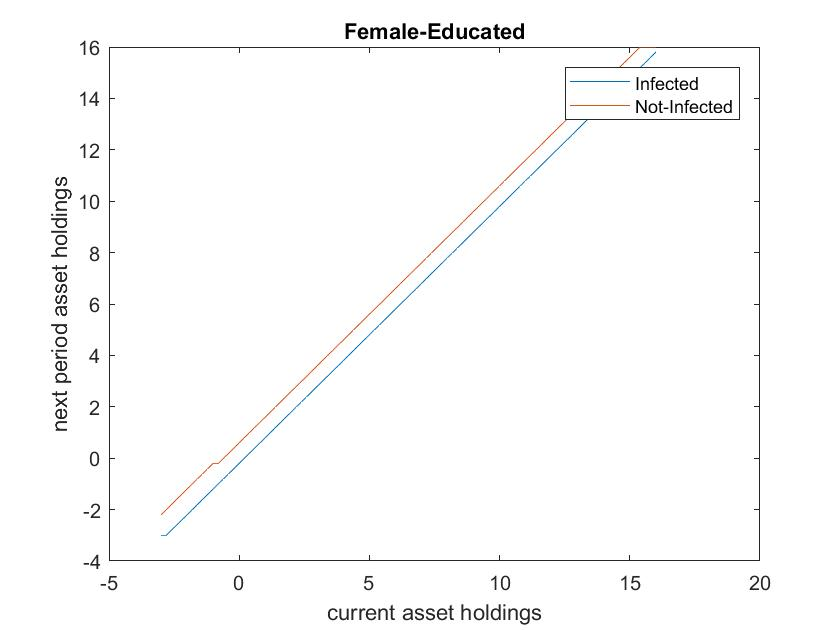
\includegraphics[width=1.3\textwidth]{miopicss/fig3a.jpg}
      
    \end{subfigure}
    \hfill
      \begin{subfigure}[b]{0.45\textwidth}
        \centering
        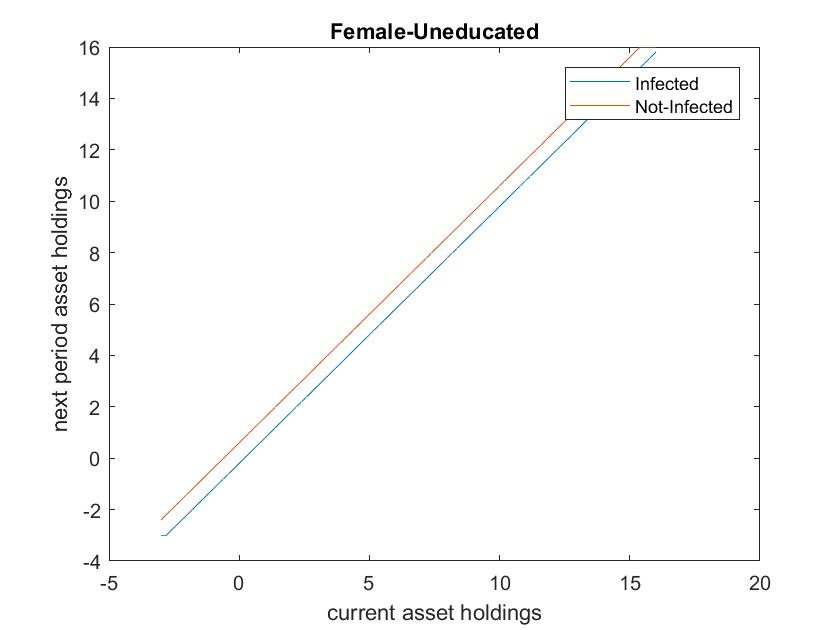
\includegraphics[width=1.2\textwidth]{miopicss/fig4a.jpg}
       
    \end{subfigure}
    
\end{figure}


\end{frame}

\begin{frame}
\frametitle{Results}

\begin{figure}
  \centering
  \caption{}
    \begin{subfigure}[b]{0.4\textwidth}
        \centering
        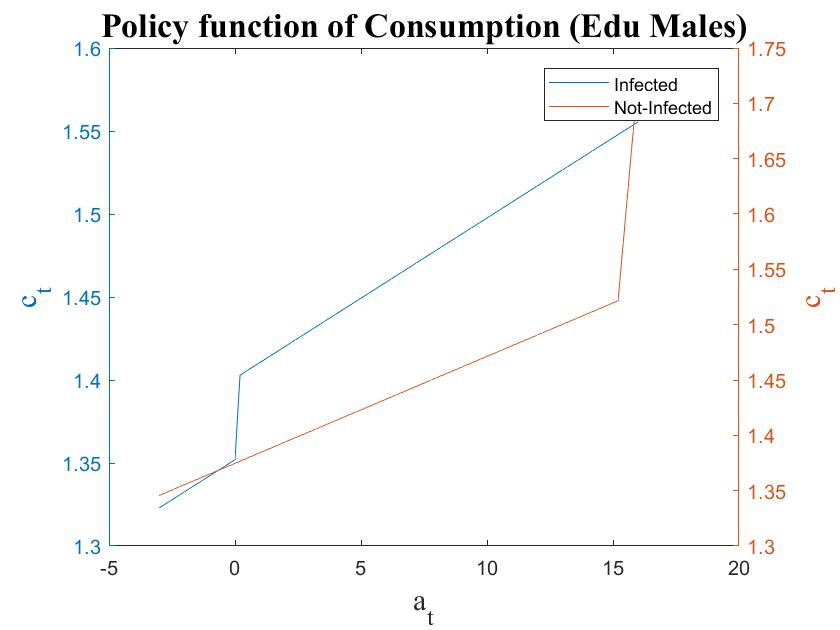
\includegraphics[width=1.3\textwidth]{miopicss/fig5a.jpg}
      
    \end{subfigure}
    \hfill
      \begin{subfigure}[b]{0.45\textwidth}
        \centering
        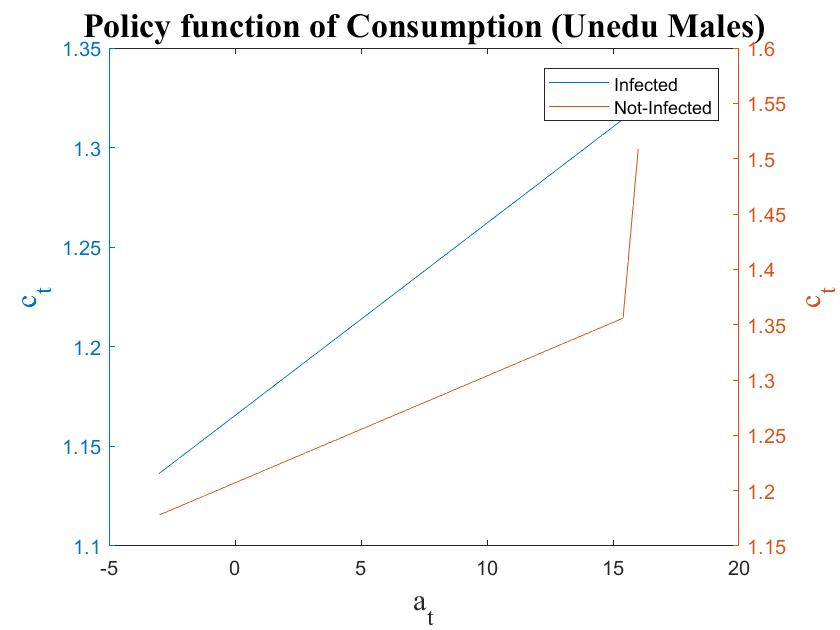
\includegraphics[width=1.2\textwidth]{miopicss/fig6a.jpg}
       
    \end{subfigure}
    
\end{figure}


\end{frame}

\begin{frame}
\frametitle{Results}

\begin{figure}
  \centering
  \caption{}
    \begin{subfigure}[b]{0.4\textwidth}
        \centering
        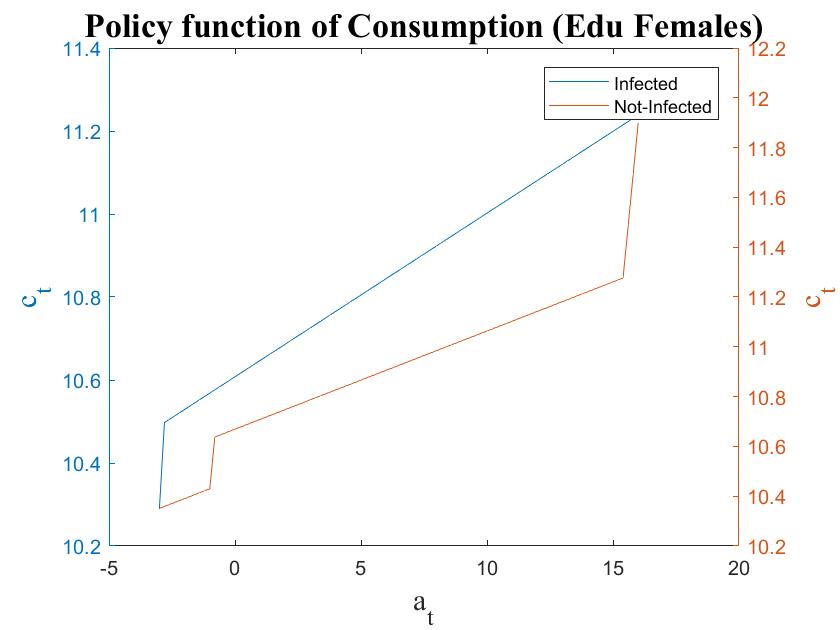
\includegraphics[width=1.3\textwidth]{miopicss/fig7a.jpg}
      
    \end{subfigure}
    \hfill
      \begin{subfigure}[b]{0.45\textwidth}
        \centering
        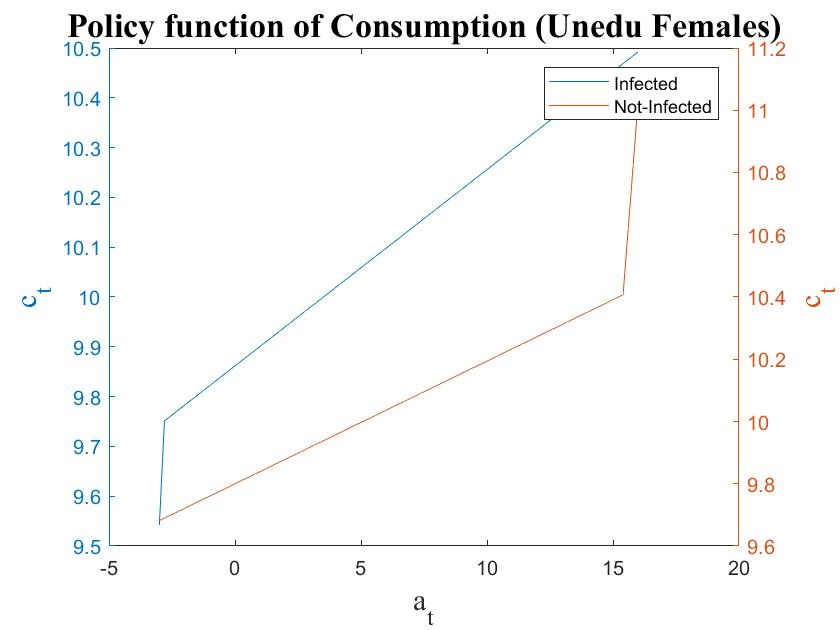
\includegraphics[width=1.2\textwidth]{miopicss/fig8a.jpg}
       
    \end{subfigure}
    
\end{figure}


\end{frame}

\begin{frame}
\frametitle{Results}

\begin{figure}
  \centering
  \caption{}
    \begin{subfigure}[b]{0.4\textwidth}
        \centering
        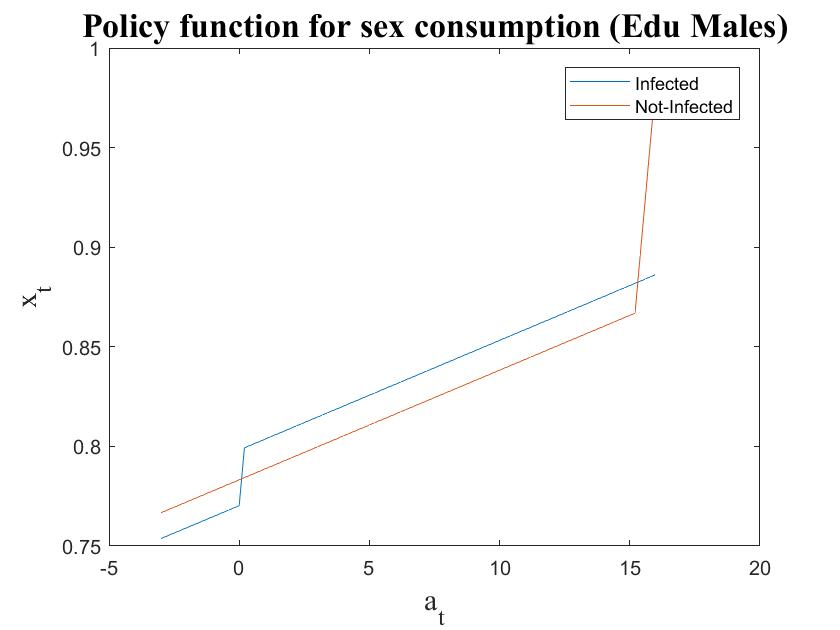
\includegraphics[width=1.3\textwidth]{miopicss/fig9a.jpg}
      
    \end{subfigure}
    \hfill
      \begin{subfigure}[b]{0.45\textwidth}
        \centering
        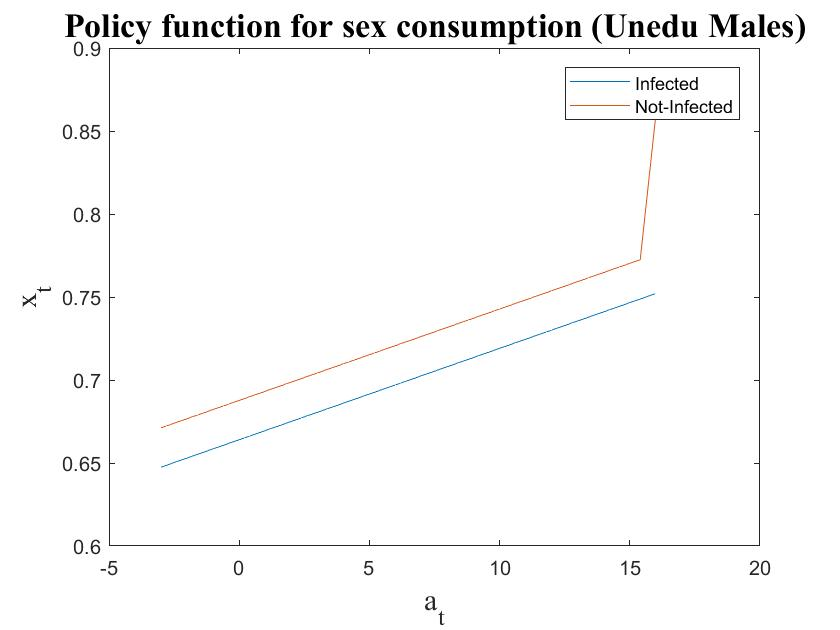
\includegraphics[width=1.2\textwidth]{miopicss/fig10a.jpg}
       
    \end{subfigure}
    
\end{figure}


\end{frame}

\begin{frame}
\frametitle{Results}

\begin{figure}
  \centering
  \caption{}
    \begin{subfigure}[b]{0.4\textwidth}
        \centering
        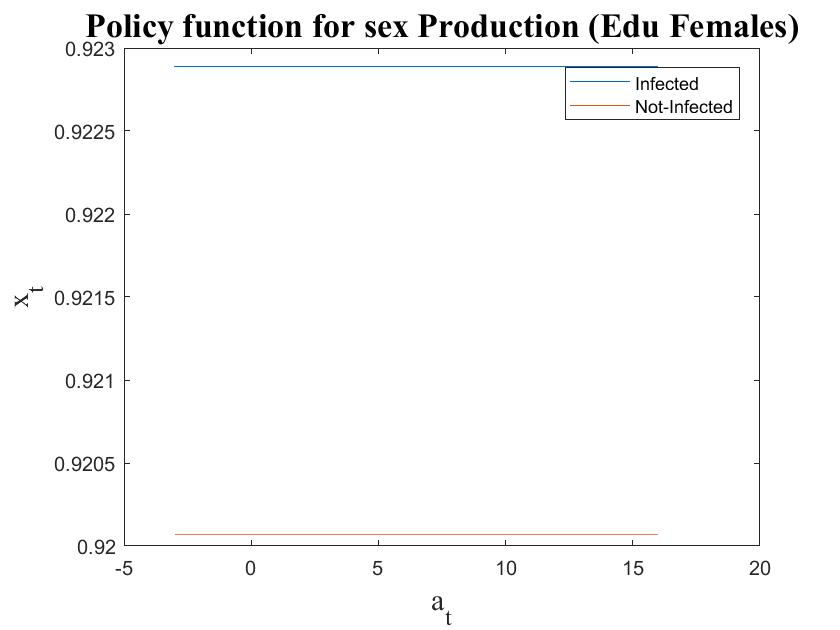
\includegraphics[width=1.3\textwidth]{miopicss/fig11a.jpg}
      
    \end{subfigure}
    \hfill
      \begin{subfigure}[b]{0.45\textwidth}
        \centering
        \includegraphics[width=1.2\textwidth]{miopicss/fig12a.jpg}
       
    \end{subfigure}
    
\end{figure}
\end{frame}
\end{comment}


\section{Results}
\subsection{}
\begin{frame}

\frametitle{Results: Policy functions}

\begin{figure}
  \centering
  \caption{Extramarital risky sex consumption \underline{\textbf{educated}} sex buyers: Myopic vs Maturity}
    \begin{subfigure}[b]{0.45\textwidth} \caption{Myopic Stage}
        \centering
        \includegraphics[width=1.2\textwidth]{FIG9a.png}
      
    \end{subfigure}
    \hfill
      \begin{subfigure}[b]{0.45\textwidth}\caption{Maturity}
        \centering
        \includegraphics[width=1.2\textwidth]{FIG9.png}
       
    \end{subfigure}
    
\end{figure}
\end{frame}

\begin{frame}

\frametitle{Results: Policy functions}

\begin{figure}
  \centering
  \caption{Extramarital risky sex consumption \underline{\textbf{less educated}} sex buyers: Myopic vs Maturity}
    \begin{subfigure}[b]{0.45\textwidth} \caption{Myopic Stage}
        \centering
        \includegraphics[width=1.2\textwidth]{FIG10a.png}
      
    \end{subfigure}
    \hfill
      \begin{subfigure}[b]{0.45\textwidth}\caption{Maturity}
        \centering
        \includegraphics[width=1.2\textwidth]{FIG10.png}
       
    \end{subfigure}
    
\end{figure}
\end{frame}

\begin{frame}
\frametitle{Calculating the HIV education gradient for Malawi\\using data generated by the model:}
A linear probability model:
\begin{align*}
y_{i,t}=\alpha_{2}+\sum_{t>2}\alpha_{t}\mathbf{1}_{t}+(\gamma_{2}+\sum_{t>2}\gamma_{t}\mathbf{1}_{t})edu_{i,t}+\epsilon_{i,t}
\end{align*}
\begin{itemize}
\item Where $i$ indexes the individual $i\in \{1,...,N\}$ 
\item $t$ indexes the stage of the epidemic $t\in \{2,3,4\}$
\item $y_{i,t}$ is the HIV status of individual $i$ living in stage of the epidemic $t$
\item $edu_{i,t}$ is the education status of the individual $i$ in stage $t$. 
\item And $E(\epsilon)=0$ and $Var(\epsilon)=\sigma^{2}$
\end{itemize}
\end{frame}

\begin{frame}
\frametitle{Calculating the HIV education gradient for Malawi}
\begin{Large}
Calculation:
\begin{itemize}
\item Education gradient:
\begin{itemize}
\item \textit{Myopic stage}: $\gamma_{2}$
\item  \textit{Maturity stage}: $\gamma_{2}+\gamma_{3}+\alpha_{3}$
\item  \textit{ARTs stage}: $\gamma_{2}+\gamma_{4}+\alpha_{4}$
\end{itemize}
\end{itemize}
Interpretation:
\begin{itemize}
\item  Finishing secondary education changes the probability of HIV infection by $x \%$. Where $x$ is the HIV education gradient of the respective stage.

\end{itemize}
\end{Large}
\end{frame}

\begin{frame}
\frametitle{Estimation Results}
\begin{figure}
  \centering
  \caption{HIV education gradient for Malawi}
   \includegraphics[width=0.6\textwidth]{edugrad.png}
 \end{figure}

\end{frame}
\begin{frame}
\frametitle{Estimation Results}
 \begin{table}[H]
 \centering
 \caption{HIV-education gradient by stage of the epidemic and by gender($\%$)}
\label{gredient}
\begin{tabular}{>{\arraybackslash}m{6cm}|c|c|c}
\hline
 \textbf{HIV-Education Gradient}& \textbf{Total} & \textbf{Males}& \textbf{Females} \\
 \hline\hline
 Stage 2($\gamma_{2}$)& $2.9$ & $4.41$& $2.42$\\
 [0.25em]
 Stage 3($\gamma_{2}+\alpha_{3}+\gamma{3}$)&$-1.45$ & $-0.60$& $-1.80$ 
 \\ 
 [0.25em]
  Stage 4($\gamma_{2}+\alpha_{4}+\gamma{4}$)
 & $-3.16$& $-3.39$& $-0.79$\\
 \hline\hline
\end{tabular}
\end{table}

\end{frame}

\begin{frame}
\frametitle{Results: HIV Education gradient}

\begin{figure}[H]
\centering
\begin{minipage}{.5\textwidth}
 \centering
 \captionof{figure}{HIV-education gradient\\ total}
%\begin{tabular}{l}
\includegraphics[width = 1\linewidth, height = 0.5\textheight]{fig_grad1.png}
\label{fig_grad1}
\end{minipage}%
\begin{minipage}{.5\textwidth}
\centering
\captionof{figure}{HIV-education gradient\\ by gender}
\includegraphics[width = 1\linewidth, height = 0.5\textheight]{fig_grad2.png}
\label{fig_grad2}
\end{minipage}
\end{figure}


\end{frame}



\section{Conclusions}
\begin{frame}
\frametitle{Conclusions}
\begin{itemize}
   		\item \textbf{Results:}
  		 \begin{itemize}
         \item The HIV education gradient for Malawi is U shaped. This is more notorious for females than for men.
  			 \item The education explains HIV exposure positively across the first stage of the HIV epidemic, it then turns negatively during the second and last stages.
   		\end{itemize}
        \item \textbf{Policy implications:}
  		 \begin{itemize}
  			 \item Targeted intervention across education groups and its timing is crucial for the effectiveness of HIV prevention policies.
   		\end{itemize}
    
   		
    
  \end{itemize}
\Huge{\centerline{Thanks for your attention}}
\end{frame}






\end{document}
